\chapter{Related Work}

The TTS conversion is not a new field and people have been working on this field before electronic
signal processing techniques. In beginning, people tried to build machines which were used to
create human sound. After the development of computers, better systems were built using different
techniques. In \cite{swetha2013text}, basic speech synthesizing technique
which works by concatenation of small recorded speech segments called phonemes to form
complete speech are discussed. Each word is first divided into syllables and then pronunciation for each syllable
is concatenated in order to get pronunciation for whole word. This concatenated word has some
delay between pronunciations of each syllable which is removed and as a result, final
pronunciation of that word is obtained. Problems like Text Preprocessing, Pronunciation and
Prosody makes it difficult. In Text Preprocessing, digits and abbreviations are converted to full
words. Other problem is guessing correct pronunciation of a word. For example, word “lives” has
different pronunciation in “He lives in Lahore” and “He saved two lives”. To create naturalness in
sound, stress and intonation are applied to the input text which is also a very complex task.


A rule based technique is designed in \cite{elovitz1976automatic}. The dataset is developed by extracting
50,000 words from standard Corpus, Corpus of Present-Day Edited American English i.e. Brown
corpus \cite{ku1967computational}. The system gave accuracy of about 93\%. A more
improved system was proposed in \cite{carlson1982multi} and \cite{klatt1982klattalk}.


Dictionary and rule based approach is used in \cite{liberman1992text} where 1000,000 words were used for training model. A TTS system with
prosody and concatenative speech parameters that were extracted through use of probabilistic
learning methods in \cite{huang1996whistler}. A formant and Concatenative synthesis is developed in \cite{huang1997recent}
where small segments of phonemes were concatenated to form whole speech. A training database
was used contains about 6,000 phonetically balanced sentences recorded in natural style. In \cite{hunt1996unit}, linear regression and unit selection 
based speech synthesis is designed using ATR Japanese database.


Statistical parametric speech synthesis is another approach which uses parameters to describe
speech. In this technique, model is learned from speech data. This technique works better than
concatenative technique. In \cite{merritt2013investigating}, author discussed shortcomings of concatenative
synthesis and why Hidden Markov model based technique is better than concatenative.

A multi-dimensional Gaussian distribution based Hidden Markov model based Statistical parametric speech synthesis system was developed in
\cite{yoshimura1998duration}.  In this technique, decision tree based context clustering is used for duration models clustering. The contextual factors are also considered with phone identity factors in this paper. Mel-cepstral coefficients are
calculated and model is trained by these coefficients. State of the context dependent is clustered using decision tree based
context clustering technique \cite{odellj.j1995}. In state duration modeling, multi-dimensional Gaussian distributions are
used to model Hidden Markov model. After estimation of duration models, using decision tree based clustering techniques,
they are clustered. By traversing decision tree, all contexts can be searched. Contextual factors which effects timing of
events in speech are also taken into account and resultant speech shows that it has good quality and natural timing. For testing
of system, 450 sentences of Japanese are used for training of system. Sampling of speech signal is done at 16 kHz. Feature
vector is composed of 25 mel-cepstral coefficients. There were 3030 states and 2984 distributions in output of the system.
The listening tests show that synthesized speech has good quality and it has natural timing even if speaking rate is changed to
some degree.

A similar system is designed in \cite{tokuda2000speech} using Hidden Markov Model and evaluated it by taking input
from Japanese database and by generating feature vector of those sentences and compared with
original speech. The parameters in this system are generated with Hidden
Markov model. The state sequence fully or partially is hidden due to which iterates algorithm for parameter generation and
forward-backward algorithm for the situation where state sequence is provided. This algorithm, from multi-mixture HMMs,
can generate clear formant structure.


A Hidden Markov model and unit selection based system is proposed in \cite{tokuda2002hmm} in which model is trained with speech database containing 
recorded speech as training data and some parameters (excitation and spectral) are extracted. These parameters are modeled by context dependent HMM. To find
accurate model parameters, decision tree based context clustering is used. The parameters are then used to generate speech
signals. These parameters can be used to control speech characteristics. In \cite{harashima2006review}, Hidden Markov model and rule based approach is applied 
on voices taken from e-learning courses and online lessons for dataset creation and tested by
generating voices and given as input to students to interpret it.


Corpus based approach for Expressive Prosody Modeling is applied in \cite{eide2004corpus} in which
manually produced dataset was used. To evaluate the synthesized
speech, the output is given for testing to 32 native English speakers. For bad news, good news and
for yes/no the accuracy is 70.2\%, 80.3\% and 84\% respectively


Tones and Break Indices ToBI are discussed on American English in \cite{pitrelli2004tobi}. Majorly
bi-gram and tri-gram were used to predict the occurrences of particular word or letter. Analysis
was performed by multiple techniques. The corpus was divided into following five yes-no
questions, either-or questions, other questions (hereafter, “wh-questions”), exclamations, and other
declarative sentences categories for the analysis purpose. Analysis by word frequency count
produced not good results and the reason was that the data was of variant types. The results show
that professional speakers produces better and informative prosodic events as compared to
ordinary speakers.

A TTS system for Azerbhaijani language using concatenative
synthesis in \cite{aida2010main} where small recordings were concatenated to make speech waveform.


Hidden Markov model based approach is used in \cite{baloyi2012text} to construct
speech synthesizer for Xitsonga which is an African language. The system received acceptability
of 92.3%.


TTS system for Fon language is designed in \cite{dagba2014text} using Multisyn algorithm
which consists of Natural Language Processing (NLP) and Digital Signal Processing (DSP)
modules. NLP consists of segmentation, Letter-to-Sound conversion and back-off rules module.
Back-off rules are applied when input text contains some characters that are not in us know
characters. DSP module than choose required unit from database of units are concatenate them to
form complete speech signals.


In \cite{ganai2016text}, hybrid text to speech converter is developed by
concatenating benefits of HMM based TTS system and waveform based TTS system. System is
developed using Matlab, a library of phoneme and their sound is created and waveform of audio
and audio itself is generated using these libraries.


A more advance technique in Neural Network based technique as it works better than Hidden
Markov model based technique. Time domain neural networks with
database containing sounds of words called phonemes is used in \cite{karaali1998text}. The basic flow of the system involves
speech recording, speech labelling, voice coder and input processing using Time Delay Neural
Network. The figure \ref{fig:Time Domain Neural Network based TTS System} shows the block diagram of system.

\begin{center}
\begin{figure}[hbtp]
\centering
  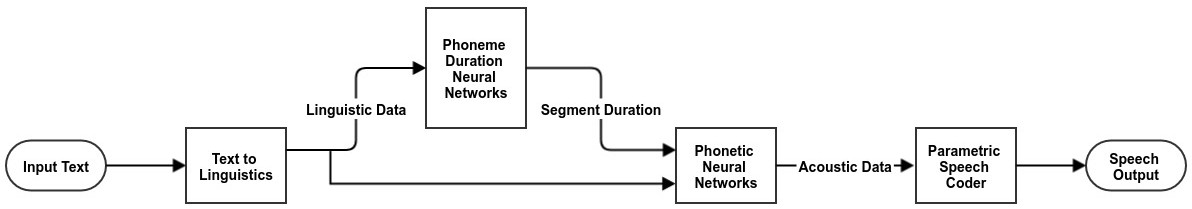
\includegraphics[width=\linewidth]{images/time_domain_neural_network.jpg}
  \caption{Time Domain Neural Network based TTS System}
  \label{fig:Time Domain Neural Network based TTS System}
\end{figure}

\end{center}

Neural network based techniques are used to learn features automatically during training along with the combination of various techniques 
like linear regression and neural network in \cite{yoshimura2016hierarchical}. Dataset of all previous Blizard Challenges \cite{blizzard_2009_corpus} and
afterwards up to 2013 were used. Model was evaluated using 5-fold cross validation. The given model gave0.11\% and 0.17\% error for LR+LR and LR+NN 
respectively.

Deep Neural Networks is applied in place of Hidden Markov model in \cite{ze2013statistical} as HMM
based system cannot model complicated context dependencies. Deep Neural Networks (DNN) can
cover limitations in HMM based system and can also outperform HMM based system. 

Recurrent Neural Networks (RNN) is applied in \cite{fan2014tts} by using the Bidirectional Long
Short Term Memory (BLSTM) with dataset consisting of 5000 training utterances and 200
utterances for testing the system. Whole recording was done in voice of female native speaker.
Objective and subjective evaluation measures are used to find distortion between natural and
synthesized speech and quality respectively. The preference results that hybrid system is better as
hybrid gave 44\%, 59\% and 55\% accuracy whereas neural network, HMM and DNN gave 29\%,
22\% and 20\% accuracy respectively.


Recurrent Neural Network (RNN) is used in \cite{muthukumar2016recurrent} for filter for
synthesis. Apart from that a novel approach was also used for training of Classification and
Regression Tree jointly instead of training all these independently.


Neural Networks is used in \cite{wu2016merlin} with dataset consisting of 328 hours was collected in
voice of native 1506 speakers. The model is tested by giving 20 sets of randomly selected from
evaluation set and asked them to rate output of each set between 0 and 100.


For Urdu Language, \cite{saleem2002urdu} and \cite{urdu_text_preprocessing} described Natural
Language Processing (NLP) unit for Urdu TTS. NLP unit is divided in two parts called as preprocessing and phonological processing unit. Pre-processing unit converts number, date and time
into their respective literal strings. For example, 100 and 5-11-2002 will be converted into \texturdu{سو} and \texturdu{پانچ نومبر دو ہزار دو} respectively. Special symbols like \$ and & are also handled in pre-processing unit. Last stage of pre-processing unit is grapheme into phoneme convertor. Phonological
processing unit contains syllable marker which marks syllable boundaries and stress and
intonation markers mark stress and intonation. A speech corpus is developed using 10 hours recorded speech of professional 
speaker containing of 1036 sentences in \cite{mumtaz2016break}. Globalphone which is a database of multilingual types is elaborated in \cite{schultz2002globalphone}. This
database contains high quality voice vocabulary which can be used for voice recognition and text to speech system. It
contains dataset of consisting more than 300 hours in voice of 1500 native speakers. It mainly cover English, Arabic,
Japanese, Turkish and 11 more languages. Scientific work done on Urdu language is limited mainly due to the reason that
there is not enough material related to phonetic strings are available for Urdu. 

In \cite{urdu_tts_db_kashif2015}, Neural Networks consists of feed forward network, back propagation for weight updation is used to generate 
speech synthesis system for Urdu. An interface is designed and tested. Mean Square Error of designed system is used as performance parameter. 
The MSE is 0.00867 of proposed system. A large database consists of 59 Urdu characters, vowels and numbers is created for this system. The designed model only
produces synthetic sound of single character. In future, urdu sentences are added to generate output in the form of full text.


In \cite{saleem2002urdu} consonantal and vocalic sounds for Urdu Language is discussed . Bi-Lingual Text to Speech Synthesis 
System for Urdu and Sindhi is designed in \cite{shah2004bi} using
bilingual hybrid knowledge based approach by using concatenated synthesis method which is capable of providing high quality 
Urdu and Sindhi speech. This system can be further expanded to include sensitive and visual text-to-speech (VTTS) policies in future.

(Hussain, S.
2005) discussed Phonological Processing unit for Urdu language in detail. This module applies
letter to sound rules, syllabification to the normalized text. This is followed by stress and intonation
marker. Statistical based part of speech tagger for
Urdu language is discussed in \cite{anwar2007statistical}. The model is evaluated by comparison of unigram, bigram and backoff
experiments with small and large tag sets. t-test, POS accuracy are used to measure performance.

Problems in Urdu segmentation are discussed for Urdu in \cite{durrani2010urdu}. Clause boundary identification is discussed in 
\cite{parveen2011clause} using classifier
and clause markers in Urdu language using conditional Random Field as a classifier. HMM based TTS system for
Urdu language using HTS toolkit is designed in \cite{ahmed2014hmm} and \cite{nawaz2014hidden}. 

% \section{Techniques used for TTS}

% \subsection{Concatenative Synthesis Model}
Concatenative speech synthesis is the model of speech synthesis where waveform is generated using concatenation of small units. In \cite{lemmetty1999review} the process of speech synthesis is divided into High-level and Low-level synthesis. In High-level, text is converted into phonetic strings. Low-level synthesis process is done by Articulatory, Concatenative and Formant based synthesis. In formant based speech synthesis, resonances in the vocal tract is modeled and this technique was widely used in
past. In concatenative synthesis, prerecorded speech samples are concatenated to form complete speech signals \cite{pickett1999acoustics}.

This IBM Expressive TTS System amazingly produced good results not only on neutral sentences and conditions but also
including good news, bad news and questions. In addition to this SSML made it capable for end users to add their customized
expressions to our system. Based on desired expressions in sentences the final audio output includes those expressions for
conveying meaningful messages.

A new text to speech synthesis system is introduced in \cite{donovan1995improvements} which used context-dependent Hidden Markov Model
for defining set of subphone units This system uses context-dependent Hidden Markov Model for defining set of subphone units. These subphone units are then used in concatenation synthesizer. The training data is one hour recorded speech which is used for getting required parameters. TD-PSOLA waveform concatenation synthesizer is then used to generate pronunciation using these parameters. The synthesized speech imitates the voice of the speaker used to record the preparing database. This system uses automatic statistical processes to extract segments of speech from large speech carpus. Desired sentence is produced by concatenation of small
segments of speech. Hidden Markov model is trained and used for segmentation of speech database into HMM-state-sized
units. A decision tree is constructed by using phonetic context labels which is used for clustering of the training speech into
acoustically self-comparable grouped states. This process helps to find most important context effects. The string to be
converted into speech is first converted into sequence of phonetic strings which then with the help of decision tree, it is
converted to speech segments. Modified Rhyme Tests \cite{house1965articulation} were used to compare system
with other. Six listeners were used with each give an answer sheet and they have to mark word from list of provided words
which is played during test. The MRT error rate for test was 5.0\% and standard error rate was 0.47\%.


Hidden Markov model is used for training of the model. The dataset used for training of model is recorded speech. Four datasets are used in which are termed as M2, M3, F1 and F2 where M stands for Male and F stands for female. Six listeners evaluate output produced by model. Error rate is used as measure of performance. 
The MRT error rate for test was 5.0\% and standard error rate was 0.47\%. Segment selection algorithm used in the system can be improved where segments in each state would be available in speech synthesis process. Dynamic programming can be used to find optimal segment sequence.
\\ \\
A system has been proposed where phoneme HMM is used to model spectra sequence in \cite{masuko1996speech}.
\\ \\
The statisticalparametric speech synthesis system can change voice characteristics of speech by speaker adaptation technique \cite{tamura1998speaker} and speaker interpolation technique \cite{yoshimura2001speaker}.